\section{多电子原子}

\begin{quotation}
“求知是所有人的本性。人都是由于惊奇而开始哲学思维的,一开始是对身边不解的东西感到惊奇,继而逐步前进,而对更重大的事情发生疑问,……”\qquad 亚里士多德
\end{quotation}

\subsection{中心力场近似}

多电子原子的哈密顿量可写为:

\begin{equation}\label{Many electrons atom}
H = \sum\limits_i {\left( { - \frac{{\hbar ^2 }} {{2m_e }}\nabla
_i^2  - \frac{{Ze^2 }} {{4\pi \epsilon _0 r_i }}} \right) + \mathop
{\sum \sum }\limits_{i < j} \frac{{e^2 }} {{4\pi \epsilon _0 \left|
{\vec r_i  - \vec r_j } \right|}}}
\end{equation}


由于“电子-电子”间相互作用的存在,薛定谔方程$H\psi=E\psi$——这里的$\psi$是$\psi(...,\vec
r_i,...)$——原则上无法严格求解。
我们的思路是取“单电子图景”,即假设电子在某个有效场$V(r)$的作用下运动,
这个有效场不仅包括电子和原子核($Ze$)的库伦势,还包括电子与除它自己外所有其他电子的相互作用。
这样,在形式上我们就不需要求解包含“电子-电子”相互作用项的薛定谔方程$H\psi=E\psi$,
我们只需求解$N$个在有效场中运动的单电子薛定谔方程。

对第$i$个电子,假设单电子波函数为:$\phi_i(\vec
r_i)$,我们需要求解如下单电子薛定谔方程($i = 1 \to N$):

\begin{equation}\label{Effective SE}
    \left( -\frac{\hbar^2}{2m_e} \nabla_i^2 + V(r_i) \right)
    \phi_i(\vec r_i) = E_i \phi_i(\vec r_i)
\end{equation}

总的能量本征值为:$E=\sum \limits_i E_i$。



我们不知道有效场$V(r)$的具体形式,但我们假设$V(r)$是球对称的,即所谓中心势场(Central
Field),对中心势场而言,我们可以对$r$和$\theta,
\phi$分离变量,即把波函数表示为矢径部分和角度部分乘积的形式,$\phi_i(\vec
r_i) = R_{n_i l_i} (r_i) Y_{l_i m_i}(\theta_i,\phi_i)$。

多电子系的波函数可写成各个单电子波函数“连乘”的形式,即:$\psi(...,\vec
r_i,...) = \prod \limits_i \phi_i(\vec r_i)$。

假设我们已经知道了波函数$\psi(...,\vec r_i,...)$,即$\{ \phi_i(\vec
r_i) \}$,我们可这样计算有效场:


\begin{equation}\label{Effective Field}
    V(r_i)=\frac{-Ze^2}{4\pi \epsilon_0 r_i} + \sum \limits_{j \ne i}
    \left\langle \frac{e^2}{4\pi \epsilon_0 \left| \vec r_i - \vec r_j \right|}  \right\rangle
\end{equation}


这里的$\left\langle ... \right\rangle$是对$\psi(...,\vec
r_i,...)$计算的,即对该$\psi$求量子力学平均,因此这种做法也叫“平均场近似”。


现在我们可以这么求解多电子原子的问题,先假设一个波函数$\{\phi_i^{(0)}\}$及对应能量本征值$\{E^{(0)}_i\}$
(比如可用氢原子的波函数),求出平均场$V^{(1)}(r_i)$,再代入薛定谔方程(\ref{Effective
SE})求出新的波函数$\{\phi_i^{(1)}\}$和新的能量本征值$\{
E^{(1)}_i\}$,如此一直进行下去,直到波函数和能量本征值收敛为止,比如:$E^{(n)}_i
- E^{(n-1)}_i \to 0$。

这样的“平均场近似”\index{Mean field: 平均场}也叫做“自洽的平均场近似”,该过程示意为:



\begin{equation*}
    \{\phi_i\} \to \left\langle V(r_i) \right\rangle
    \to \{\phi_i\} \to \left\langle V(r_i) \right\rangle \to
    ...
\end{equation*}


讨论:

\begin{itemize}
  \item 我们假设有效场是中心力场,所以单电子薛定谔方程的解仍然可按矢径部分和角度部分分离变量,
对角度部分而言它的解和氢原子的解完全相同,都是$Y_{lm}(\theta,\phi)$,
对矢径部分,由于有效场$V$不同于库伦势,所以$R_{nl}$的解不同于氢原子的解,
但我们仍可说$n-l-1$对应于节点数,只是能量本征值发生了变化,由氢原子的$E_n$形式变成了$E_{nl}$。

  \item
  由于电子的自旋是$1/2$,所以实际的波函数比我们现在讨论的还要复杂,
  每个单电子的波函数都要写成轨道部分$\phi(\vec r_i)$和自旋部分$\chi(s_z)$的乘积$\phi(\vec r_i)\chi(s_z)$的形式。

  \item
  研究氢原子时引入的量子数$n,l,m,s_z$对研究多电子原子也适用,
  单电子波函数可表示为$R_{nl}(r)Y_{lm}(\theta,\phi)\chi(s_z)$的形式。

\index{Pauli exclusion principle: 泡利不相容原理}

  \item 在量子力学中,由于电子是全同费米子,多电子波函数$\psi(...,\vec
  r_i,...;...,s_{iz},...)$最终还需要反对称化(即当交换任意两个电子的宗量时,
  包括自旋宗量,也包括位置宗量,满足波函数交换反对称:$\Psi(1,2)=-\Psi(2,1)$),
  也是因为这个原因,多电子原子需要满足“泡利不相容原理”,即在多电子原子中,
  不存在两个电子具有完全相同的量子数(如:$n,l,m,s_z$)。

\end{itemize}


\subsection{光谱记号}

\subsubsection{电子组态}


在“中心力场”近似下,相同$n,l$的电子具有相同的能量,我们把相同$n$称之为壳层(shell),
相同$nl$称之为亚壳层(sub
shell),电子依次由低到高填充的构形可表示为:$nl^{N}n'l'^{N'}$的形式,
这里$N$表示占据亚壳层$nl$的电子数。这种表示原子中各壳层电子填充的方式叫做``电子组态''(configuration)\index{Configuration: 电子组态}。

例:碳(carbon)原子有6个电子,碳的基态组态(ground state
configuration)是:$1s^2 2s^2 2p^2$

对于充满的壳层或亚壳层而言,总的轨道角动量(用$L$表示)和总的自旋角动量(用$S$表示)为0。
但对部分充满的亚壳层而言,相同的组态(configuration)可能对应不同的$L$和$S$。

\subsubsection{L-S耦合和光谱记号}

由于原子中的电子存在着轨道运动和自旋运动,
所以原则上说电子存在着由于轨道运动所导致的非零磁矩和由于自旋运动所导致的非零磁矩,
除此之外,原子核还有核磁矩。我们可以把这些磁矩间的相互作用看作是微扰,予以考虑。

我们暂时不考虑核磁矩, 对电子而言, 存在着两种方案,
一种是对较轻原子适用的$L-S$耦合 (较轻原子, 一般指比Fe“轻”的原子,
不考虑狭义相对论效应, 总轨道角动量$L$和总自旋角动量$S$是好量子数),
另一种是对较重原子适用的$j-j$耦合(较重原子, 必须考虑狭义相对论效应,
每个电子的$\hat l$和每个电子的$\hat s$存在较强耦合\footnote{$U
\propto Z^4$, 这里Z是原子序数, 参考:杨福家《原子物理学》,
pp170.})。我们暂时先只讨论$L-S$耦合。

对$L-S$耦合而言,所有电子的轨道角动量相加得到总轨道角动量$\vec
L=\sum \limits_i \vec
l_i$。所有电子的自旋角动量相加得到总自旋角动量$\vec S =\sum
\limits_i \vec s_i$。然后$L$和$S$相加得到总角动量$\vec J = \vec L +
\vec S$。

例:考虑被电离掉两个电子的$O_{III}$,组态是:$1s^2 2s^2
2p3d$,求:$L,S,J$。

解:首先满壳层,和满亚壳层的贡献为零。只需考虑$2p3d$。

对$2p$电子而言,$l_1=1$, $s_1=1/2$

对$3d$电子而言,$l_2=2$, $s_2=1/2$

$\vec L = \vec l_1 + \vec l_2$, $L = 3,2,1$

$\vec S = \vec s_1 + \vec s_2$, $S = 1, 0$

$\vec J = \vec L + \vec S$,


\begin{center}

\begin{tabular}{|c|c|l|c|l|}
  \hline
  % after \\: \hline or \cline{col1-col2} \cline{col3-col4} ...
  L & S & J & 项(Term) & 能级(Level) \\
\hline

  3 & 1 & 4,3,2 & $3F^o$ & $^3F^o_4, ^3F^o_3, ^3F^o_2$ \\
  3 & 0 & 3 & $^1F^o$ & $^1F^o_3$ \\
  2 & 1 & 3,2,1 & $^3D^o$ & $^3D^o_3,^3D^o_2,^3D^o_1$ \\
  2 & 0 & 2 & $^1D^o$ & $^1D^o_2$ \\
  1 & 1 & 2,1,0 & $^3P^o$ & $^3P^o_2,^3P^o_1,^3P^o_0$ \\
  1 & 0 & 1 & $^1P^o$ & $^1P^o_1$ \\
  \hline
\end{tabular}

\end{center}

讨论:

\begin{itemize}
  \item
  角动量相加,比如角动量量子数分别为$l_1$和$l_2$的两个角动量相加,
  总角动量量子数$L = l_1 + l_2, l_1 + l_2 -1, ..., \left|l_1-l_2\right|$

  \item
  项(Term)的光谱记号:$^{2S+1}L^{(o)}$,这里$2S+1$叫多重度(multiplicity),
  比如$S=0$叫单态(singlet),$S=1/2$叫双态(doublet),$S=1$叫三重态(triplet)。
  $L$用大写的$S,P,D,F,G,H,...$表示,分别对应$L=0,1,2,3,4,5,...$。$(o)$表示表示波函数的宇称(parity),
  如果波函数在空间反演变化($\vec r \to - \vec
  r$)下对称$\psi(- \vec r) = \psi(\vec r)$,称为偶宇称(even),
  反对称$\psi(- \vec r) = - \psi(\vec r)$,则称为奇宇称(odd),
  对奇宇称需要在$L$右上角注明$o$。多电子波函数的宇称可由$\sum \limits_i l_i$
  进行估算,和为偶数则宇称为偶,和为奇数则宇称为奇。
  我们可以证明,偶极跃迁只能发生在宇称不同的波函数之间。

  \item
  能级(Level)的光谱记号:$^{2S+1}L^{(o)}_J$,需要在$L$的右下角注明$J$。
  需要注意的是,$^{2S+1}L^{(o)}_J$仍然存在着简并,它对应$M_J=J,J-1,...
  -J$的$2J+1$个量子态。我们可进行验算,对$2p3d$组态,应有$2(2l_1+1)\times
  2(2l_2+1)=60$个不同的量子态。

\end{itemize}


\subsubsection{洪特定则}

相同的组态(configuration)会导致不同的项(terms),这些项可以有不同的能量。

例:氦原子($He$)

(1)考虑基态组态:$1s^2$,这是个闭合的壳层,因此$L=0$, $S=0$,
项:$^1S$, 能级:$^1S_0$。

(2)第一激发态组态:$1s2s$,

$l_1=0, l_2=0$, 因此:$L=0$;$s_1=1/2, s_2=1/2$, 因此$S=1,0$;

那么单态(Term:$^1S$,Level:$^1S_0$),和三重态(Term:$^3S$,
Level: $^3S_1$)哪个能量更低呢?

这个可通过\textbf{洪特第一定则}来判定:
\texttt{给定组态,具有最大自旋多重度的量子态能量最低}。
在这里就是三重态($^3S$)能量更低,低大约$0.80eV$。

我们可以这样来理解洪特第一定则,由于泡利不相容原理,
相同自旋量子数$s_z$的电子总是倾向于空间分离的,因此具有较低的库伦排斥能。

(3)再下一个激发态的组态:$1s2p$

$l_1=0, l_2=1$, 因此具有奇宇称。同时:$L=1$。

$s_1=1/2, s_2=1/2$, $S=1, 0$

Terms: $^3P^{o}$, $^1P^{o}$,
根据洪特第一定则,$^3P^{o}$低于$^1P^{o}$,低$0.25eV$。

Levels: $^3P^{o}_{2,1,0}$, $^1P^{o}_1$


例:碳原子


(1)考虑激发态的组态:$1s^2 2s^2 2p 3p$

只需考虑部分填充壳层的组态$2p 3p$, $l_1 = 1, l_2 = 1$, $s_1=1/2,
s_2=1/2$

$L=2,1,0$, $S=1,0$

Terms: ${}^1S, {}^3S, {}^1P, {}^3P, {}^1D, {}^3D$

(2)现在考虑碳的基态组态:$1s^2 2s^2 2p^2$

仍然有:$l_1 = 1, l_2 = 1$, $s_1=1/2, s_2=1/2$

\index{Equivalent electrons: 同科电子}

但由于两个电子都是$2p$,所以这里必须考虑“泡利不相容原理”。对于两个``同科电子''(equivalent
electrons, 即具有相同$nl$的电子),
“泡利不相容原理”意味着$L+S$必为偶数。

因此允许的项(Terms)是:${}^1S, {}^3P,
{}^1D$。${}^3P$的项具有最大自旋多重度,因此对应是基态的项。
剩下的两个项${}^1S$和${}^1D$具有相同的自旋多重度,那么哪一个能量更低呢?
这就需要用到\textbf{洪特第二定则}:

\texttt{对相同组态和相同自旋多重度,最大轨道角动量意味着更低的能量。}

我们可以这样来理解洪特第二定则,最大轨道角动量意味着“电子-电子”间角分布分的最开,
有利于降低库伦能。

因此$^1D$的能量要低于$^1S$的能量,低大约$1.42eV$,但比基态项$^3P$高$1.26eV$。

以上都没有考虑$J$的不同对能量的影响,这个分裂对$Z$较大(或不太严格地说是“较重”)的原子会越来越明显。

对项:$^3P$而言,$L=1, S=1$, $J=2,1,0$, 能级(Levels): ${}^3P_2,
{}^3P_1, {}^3P_0$。它们的高低由\textbf{洪特第三定则}给出:

\texttt{相同组态(configuration),自旋多重度($S$),和轨道角动量($L$),如果壳层少于半充满(normal
case,正常情况),具有最小$J$值的态能量更低;如果壳层多于半充满(inverted
case,倒转情况),具有最大$J$值的态能量更低。}

对碳原子来说,$2p^2$低于半充满,因此$J$小的态能量更低,即:${}^3P_0
< {}^3P_1 < {}^3P_2$。

小结:

(1)洪特第一定则:给定组态,具有最大自旋多重度($S$)的量子态能量最低。

(2)洪特第二定则:对相同组态和相同自旋多重度($S$),最大轨道角动量($L$)意味着更低的能量。

(3)洪特第三定则:相同组态,自旋多重度($S$),和轨道角动量($L$),如果壳层少于半充满,具有最小$J$值的态能量更低;

(4)洪特第四定则:相同组态,自旋多重度($S$),和轨道角动量($L$),如果壳层高于半充满,具有最大$J$值的态能量更低。


\subsection{选择定则}

\subsubsection{电偶极跃迁}

针对电偶极相互作用(electric dipole),磁偶极相互作用(magnetic
dipole),和电四极矩相互作用(electric
quadrupole),我们可以计算跃迁的选择定则。
电偶极相互作用的谱线最强,这个可由爱因斯坦$A$系数,或寿命看出:

\begin{equation*}
    \tau_{\text{dipole}} \sim 10^{-8}s, \tau_{\text{magnetic}} \sim 10^{-3}s,
    \tau_{\text{quadrupole}} \sim 1s
\end{equation*}

总寿命$\tau$将主要由$\tau_{\text{dipole}}$决定,

\begin{equation*}
\frac{1}{\tau} = \frac{1}{\tau_1} + \frac{1}{\tau_2} +
\frac{1}{\tau_3} +...
\end{equation*}


这意味着:电偶极跃迁的强度要比磁偶极强5个数量级,磁偶极跃迁又要比电四极矩跃迁强3个数量级。

下面仅针对电偶极跃迁,列出选择定则。

首先是严格的选择定则(rigorous selection
rules),只要满足以下定则,跃迁就会发生,但有些可能比较弱。

(1)$\Delta J = 0, \pm 1$, 但 $J=0 \nleftrightarrow J=0$

(2)$\Delta M_J = 0, \pm 1$

(3)宇称改变,即:$odd \leftrightarrow even$

还有一些额外的选择定则,仅针对一个电子参与的跃迁,将导致较强的跃迁,可称为
propensity rules。

(4)$\Delta S =0$

(5)仅一个电子跃迁,$\Delta n $无限制,$\Delta l =\pm 1$, 如:$2s^2
\leftrightarrow 2s2p$是允许的,但$2s^2 \leftrightarrow 2s3d$或 $2s^2
\leftrightarrow 3p^2$是不允许的。

(6)$\Delta L =0, \pm 1$, 但 $L =0 \nleftrightarrow L=0$


\subsubsection{j-j耦合}

如果每个电子自身的自旋与轨道耦合较强(即自旋磁矩和轨道磁矩间相互作用较强),
不同电子之间的耦合较弱, 每个电子的自旋角动量$\vec
s$和轨道角动量$\vec l$会先耦合形成总角动量$\vec j$,
然后单电子的总角动量$\vec j_i$继续相互耦合得到总角动量$\vec J$.
这就是``j-j耦合'', 记为:

\begin{equation*}
(s_1 l_1)(s_2 l_2)(s_3 l_3)... =(j_1 j_2 j_3 ...) =J
\end{equation*}

``j-j耦合''的选择定则是:

\begin{eqnarray*}
% \nonumber to remove numbering (before each equation)
  \Delta j &=& 0, \pm 1 \\
  \Delta J &=& 0, \pm 1; J=0 \nleftrightarrow J=0
\end{eqnarray*}



考虑电子的$sp$组态, 即一个电子处在$l=0$, 另一个处在$l=1$.
``j-j耦合'', $j_1 =1/2$; $j_2 = 3/2, 1/2$, 这样$J = 2, 1, 1, 0$,
或$(1/2, 3/2)_2$, $(1/2, 3/2)_1$, $(1/2, 1/2)_1$, $(1/2, 1/2)_0$.





\subsubsection{氦光谱}

氦有两套光谱, 一套对应的是自旋单态($2S+1=1$)之间的跃迁,
另一套对应的是自旋三重态($2S+1=3$)之间的跃迁,
在自旋单态和自旋三重态之间不存在跃迁(跃迁法则: $\Delta S =0$).
以前人们曾认为有两种氦, 具有三重态的氦称为``正氦''(Ortho),
单态的氦称为``仲氦''(Para).

除了基态$1^1S_0$(电子组态: $1s^2$), 在He原子中存在着亚稳态,
即能量不是最低, 但由于选择定则的限制, 这些原子态的寿命很长.
比如$2^1S_0$(电子组态: $1s2s$), 由于选择定则$J=0 \nleftrightarrow
J=0$, 所以$2^1S_0 \nrightarrow 1^1S_0$;
又比如$2^3S_1$(电子组态$1s2s$, 寿命为8000秒\footnote{Jonathan
Tennyson, Astronomical Spectroscopy, pp77;}), 由于选择定则$\Delta
S=0$, 所以$2^3S_1 \nrightarrow 1^1S_0$.

\subsection{元素周期性}

化学元素性质存在着周期性, 比如对电离能而言, 如图(\ref{periodic
ionizing energy}), 元素的电离能随着$Z$的增大呈周期性的变化.

\begin{figure}[h]
\begin{center}
  % Requires \usepackage{graphicx}
  \includegraphics[width=8cm]{Spectrum/ionizing_energy.ps}\\
  \caption{元素的电离能}\label{periodic ionizing energy}
\end{center}
\end{figure}


\subsubsection*{贯穿与屏蔽}

由于泡利不相容原理的存在, 多电子原子的性质主要是由最外层电子决定的.
考虑多电子原子中最外层的一个电子, 如果这个电子的轨道角动量$l$较大,
按旧量子论——玻尔---索末菲理论(Bohr---Sommerfeld
theory)——电子距离原子核(电荷: $Ze$)较远, 距离其他电子(电荷:
$-(Z-1)e$)也较远, 这样原子核就被其周围的电子屏蔽掉了,
有效电荷$Z_{eff}$会降低, 极限情况是$Z_{eff}=1$, 即此时能量会比较高.


如果最外层电子的轨道角动量$l$较小, 按玻尔---索末菲理论,
如图(\ref{orbital penetration}), 电子会穿透内层的电子靠近原子核,
这就是轨道贯穿, 屏蔽效应会减弱, 极限情况$Z_{eff}=Z$, 此时能量会较低.


\begin{figure}
\begin{center}
  % Requires \usepackage{graphicx}
  \includegraphics[width=8cm]{Spectrum/bohr-sommerfeld-model.ps}\\
  \caption{轨道贯穿, 相同的$n$不同的$l$, 距离原子核的远近是不同的, 即轨道贯穿的程度是不同的.}\label{orbital penetration}
\end{center}
\end{figure}


\subsubsection*{轨道填充次序}

对多电子原子, 由于电子的贯穿效应, $E_{nl}$是不同的,
$l$越小贯穿效应越大, 相应地能量也越低, 能级的排序如下:

$1s < 2s < 2p < 3s < 3p < 4s < 3d < 4p < 5s < 4d < 5p < 6s < 4f < 5d
< 6p$

由于泡利不相容原理, ``贯穿和屏蔽''效应,
多电子原子中的电子将按由低到高的次序依次填充各亚壳层,
如图(\ref{Shell subshell filling}).

\begin{figure}[h]
\begin{center}
  % Requires \usepackage{graphicx}
  \includegraphics[width=5cm]{Spectrum/subshell-filling.ps}\\
  \caption{原子能级的填充次序}\label{Shell subshell filling}
\end{center}
\end{figure}

\subsection{碱金属光谱}


对碱金属(Li, Na, K, Rb, Cs, Fr)而言, 除最外层的一个s电子外,
其他电子都形成了满壳层. 可只考虑最外层的那个s电子,
与剩余部分——带1个单位正电荷的原子实($Z=1$)——之间的相互作用.

对锂(Li, Lithium)原子而言, 基态组态$1s^22s$,
最外层电子只能由$n=3,4,...$跃迁到$n'=2$,

\begin{equation*}
\frac{1}{\lambda} = R \left[ \frac{1}{2^2} - \frac{1}{n^2} \right]
\end{equation*}

对$n'=2$, $l=0, 1$, 即有$2S$和$2P$两种情形, 由跃迁法则: $\Delta l =
\pm 1$, 存在以下几种跃迁的可能:

\begin{enumerate}
  \item $nP \to 2S$, 称为主线系(Principal series);
  \item $nS \to 2P$, 称为锐线系(Sharp series);
  \item $nD \to 2P$, 称为漫线系(Diffuse series), 又称第一辅线系;
\end{enumerate}

如果再考虑由$n=4$到$n'=3$的跃迁, 还有:$nF \to 3D$,
称为基线系(Fundamental series), 又称柏格曼线系(Bergmann series).

\subsubsection{量子缺陷}

考虑到原子实是有大小的, 最外层电子能量不再严格地反比于$n^2$,
而是会有个修正, 而且这个修正将会和角动量量子数$l$有关,
我们一般将其写为:

\begin{equation*}
E_{nl}=-R\frac{Z_{eff}^2}{(n-\mu_{nl})^2}
\end{equation*}

这里$Z_{eff}$是有效电荷, $\mu_{nl}$叫量子缺陷(quantum defect)\index{Quantum defect: 量子缺陷},
对比如Na原子($1s^22s^22p^63s$)而言, 取值如下:


\begin{table}[h]
  \centering
\begin{tabular}{|c|c|c|c|c|c|c|}
  \hline
  % after \\: \hline or \cline{col1-col2} \cline{col3-col4} ...
  $l$ & {} & $n=3$ & $n=4$ & $n=5$ & $n=6$ & $n=\infty$ \\
  \hline
  0 & s & 1.373 & 1.357 & 1.353 & 1.351 & 1.348 \\
  1 & p & 0.883 & 0.867 & 0.862 & 0.857 & 0.855 \\
  2 & d & 0.012 & 0.013 & 0.014 & 0.014 & 0.015 \\
  3 & f & - & 0.000 & 0.000 & 0.000 & 0.000 \\
  \hline
\end{tabular}
  \caption{Na原子的量子缺陷$\mu_{nl}$.}\label{quantum defects for sodium atoms}
\end{table}

讨论:

\begin{enumerate}
  \item ``贯穿效应''使有效的$n$值($n_{eff}$)变小;
  \item $n$越大, 贯穿效应越弱;
  \item $l$越小, 贯穿效应越大, 当$l \ge 3$时, 贯穿效应几乎没有了, 即$\mu_{43}\approx 0$.
\end{enumerate}

对Na原子而言, 可能存在$n=3,4,5,6,...$到$n'=3$的跃迁. 比如可能存在$3P
\to 3S$的跃迁(主线系).

\begin{figure}[h]
\begin{center}
  % Requires \usepackage{graphicx}
  \includegraphics[width=11cm]{Spectrum/line-spectra.ps}\\
  \caption{碱金属光谱}\label{spectra for potassium atoms}
\end{center}
\end{figure}


\subsubsection{碱金属双线}



如果我们观察碱金属光谱(图\ref{spectra for potassium atoms})的话,
我们会发现在Na光谱中存在着一个很明显的双线结构, 黄光, 分别是$589.6
nm$和$589.0 nm$, 对应的就是$3P \to 3S$的跃迁.

对于$3P$电子而言, $l=1$, $s=1/2$, $j$可以有两种取值, 即: $j=3/2,
1/2$. 写成原子态记号分别是: $3^2P_{3/2}, 3^2P_{1/2}$.

\subsubsection{自旋轨道相互作用}

电子自旋和轨道运动都可能导致非零的磁矩, 对$3P$电子而言,
自旋导致的磁矩$\vec \mu_s$和轨道导致的磁矩$\vec \mu_l$都不是0,
因此在自旋和轨道之间将会存在相互作用, 即在能量项中将再加一项,
对应的是自旋磁矩和轨道磁矩间的相互作用. 这个能量是:


\begin{equation}\label{spin-orbital coupling}
U =\frac{1}{4\pi \epsilon_0}\frac{Z e^2}{2 m_e^2 c^2 r^3} \vec s
\cdot \vec l
\end{equation}

这个公式可进一步被简写为:

\begin{equation*}
U = \xi(r) \vec s \cdot \vec l
\end{equation*}

对氢原子第二能级, 估算出的修正值为: $U \simeq 10^{-5}eV$数量级.

为了定量计算 $U = \left\langle \xi(r) \right\rangle \left\langle
\hat s \cdot \hat l \right\rangle = A(n,l)\left\langle \hat s \cdot
\hat l \right\rangle$, 我们需要先计算$\vec s \cdot \vec l$,
如果定义总角动量是: $\vec j = \vec s + \vec l$, 则:

\begin{equation*}
\vec j \cdot \vec j = (\vec s + \vec l)\cdot (\vec s + \vec l) =
\vec s \cdot \vec s + \vec l \cdot \vec l + 2 \vec s \cdot \vec l
\end{equation*}

要注意上式中的$\vec j, \vec s, \vec l$都是算符, 我们把它改写为:

\begin{equation*}
\hat j^2 = \hat s^2 + \hat l^2 + 2\hat s \cdot \hat l
\end{equation*}

我们希望能够求出算符$\hat s \cdot \hat l$对应的期望值(或平均值),

\begin{equation*}
\left\langle \hat s \cdot \hat l \right\rangle = \frac{\left\langle
\hat j^2 - \hat s^2 -\hat l^2 \right\rangle}{2} =
\frac{j(j+1)-s(s+1)-l(l+1)}{2}\hbar^2
\end{equation*}

把$s=1/2$, $l=l$, $j=l\pm \frac{1}{2}$分别代入上式, 得到:

\begin{eqnarray*}
% \nonumber to remove numbering (before each equation)
  \left\langle \hat s \cdot \hat l \right\rangle &=& \frac{l}{2}\hbar^2, j=l+\frac{1}{2} \\
  \left\langle \hat s \cdot \hat l \right\rangle &=&
  -\frac{(l+1)}{2}\hbar^2, j=l-\frac{1}{2}
\end{eqnarray*}

对Na原子, $A(n,l)>0$\footnote{参考: 杨福家《原子物理学》, pp169;

计算中需要用到积分:

\begin{equation*}
\left\langle \frac{1}{r^2}\right\rangle = \int_0^{\infty} (R_{nl})^2
\frac{1}{r^2} r^2 dr = \frac{Z^2}{a_1^2 n^3 (l + 1/2)}
\end{equation*}

参考: 杨福家《原子物理学》, pp131.},
$3^2P_{3/2}$的能量要高于$3^2P_{1/2}$的能量,
这其实就是``洪特第三定则''. Na原子双黄线一般被标记为:


\begin{itemize}
  \item $D_2$线, $\lambda = 589 nm$, $3p \to 3s$, $3^2P_{3/2} \to 3^2S_{1/2}$
  \item $D_1$线, $\lambda = 589.6 nm$, $3p \to 3s$, $3^2P_{1/2} \to 3^2S_{1/2}$
\end{itemize}

对应能量差为约$2 \times 10^{-3}eV$.



\subsection*{练习}

\begin{enumerate}
  \item 请写出Be的基态组态(configuration), 基态项(term),
和基态能级(level);假设Be的一个外层电子被激发到$3d$轨道,
请写出对应这个激发组态的各个项(terms)和能级(levels)。


  \item 对记号${}^4F^o_{7/2}$, $L$,
$S$和$J$分别是多少?它对应多少个不同的态?对这个项(term),
它还可以有哪些能级(levels)?

至少需要多少个电子才能够形成这个项(term)?请写出对应这个项(term)的可能的组态(configuration)。


  \item 对以下这些记号${}^1D_1$, ${}^0D_{5/2}$, ${}^3P_{3/2}$,
请分别解释它们为什么是错误的。

\begin{quote}
解:(1)${}^1D_1$, $S=0$, $L=2$, $J=2 \ne 1$; (2) ${}^0D_{5/2}$,
$2S+1 \ge 1 \ne 0$ ; (3)${}^3P_{3/2}$, $S=1$, $L=1$, $J=L+S=2,1,0
\ne 3/2$
\end{quote}


  \item 对Ca的一个组态$1s^2 2s^2 2p^6 3s^2 3p^6 3d 5p$,
  写出它的项(terms),
  根据洪特定则判断哪一项具有最低的能量。这个最低能量项(term)对应的能级(levels)有哪些?


\item 同科电子$4d^2$, 写出所有允许的原子态记号.

解: $l_1 =2$, $s_1 =1/2$, $l_2 =2$, $s_2=1/2$;

考虑$\vec S = \vec s_1 + \vec s_2$, $S = 1, 0$;

$\vec L = \vec l_1 + \vec l_2$, $L = 4, 3, 2, 1, 0$.

对同科电子, 必须考虑``泡利不相容''原理, 对两个电子$L+S$必须是偶数.

$S=1$, $L=3$, $J=4,3,2$, 因此有: ${}^3 F_{4,3,2}$;

$S=1$, $L=1$, $J = 2,1,0$, 因此有: ${}^3 P_{2,1,0}$;

$S=0$, $L=4$, $J=4$, 因此有: ${}^1 G_4$

$S=0$, $L=2$, $J=2$, 因此有: ${}^1 D_2$;

$S=0$, $L=0$, $=0$, 因此有: ${}^1 S_0$.

  \item 定性证明: 原子中电场对电子的影响要比磁场对电子的影响大得多.

  解: 电子受静电力, 大小是$e \vec E$, 电子还受洛仑兹力, 大小是: $e \vec v \times \vec B
  $. 其比值是: $\frac{e E}{ e v B}$


假设这里的电场和磁场是入射的光波导致的, E, B之间会存在定量的关系.

\begin{equation*}
    \vec B = \frac{1}{c}\hat k \times \vec E
\end{equation*}

因此:

\begin{equation*}
    \frac{e E}{ e v B} = \frac{c}{v} =\frac{1}{\alpha} \approx 137
\end{equation*}

即电场对电子的相互作用比磁场对电子的相互作用至少大100倍. 就光谱问题,
磁偶极跃迁相对于电偶极跃迁是可以忽略的.


  \item 计算${}^4D_{3/2}$态的$\vec L \cdot \vec S$.
  \item 对于$S=1/2$和$L=2$, 试计算$\vec L \cdot \vec S$的可能值.

\end{enumerate}
